%
% wavelets.tex
%
% (c) 2019 Prof Dr Andreas Müller, Hochschule Rapperswil
%
\section{Wavelets}
\rhead{Wavelets}
Das Ziel ist also, Funktionen mit Hilfe von verschobenen und skalierten
Versionen eines sogenannten {\em Mutterwavelets} $\psi(t)$ zu analysieren.
\index{Mutterwavelet}
Die Analyse spielt sich im Raum der quadratintegrierbaren Funktionen
$L^2(\mathbb R)$ ab, so dass vorausgesetzt werden muss,
dass $\psi\in L^2(\mathbb R)$.
Man stellt sich auch vor, dass $\psi$ so etwas wie ein Basisvektor ist,
daher wird verlangt dass $\|\psi\|=1$.

Diese Voraussetzungen reichen jedoch nicht.
Es stellt sich heraus, dass einfache Rekonstruktionsformeln nur zu
bekommen sind, wenn die Funktion $\psi(t)$ zusätzlich der folgenden
{\em Zulässigkeitsbedingung} genügen.
\index{Zulässigkeitsbedingung}%

\begin{definition}
Eine Funktion $\psi\in L^2(\mathbb R)$ mit $\|\psi\|=1$ heisst 
{\em Mutterwavelet} oder einfach nur {\em Wavelet}, wenn ihre
\index{Mutterwavelet}
Fourier-Transformierte $\hat{\psi}(a)$ zusätzlich die Bedingung
\begin{equation}
C_{\psi}
:=
2\pi
\int_{-\infty}^\infty \frac{|\hat{\psi}(a)|^2}{|a|}\,da < \infty
\label{cwt:zulaessig}
\end{equation}
erfüllt.
\end{definition}

\begin{beispiel}
Das Haar-Mutterwavelet
\[
\psi_{\text{Haar}}(t) = \begin{cases}
 1&\qquad 0\le t < \frac12\\
-1&\qquad \frac12 \le t < 1\\
 0&\qquad \text{sonst}
\end{cases}
\]
erfüllt die Zulässigkeitsbedingung.
Dazu muss die Fourier-Transformation von $\psi_{\text{Haar}}$ berechnet
werden.
Es gilt
\begin{align*}
\hat{\psi}_{\text{Haar}}(\omega)
&=
\frac{1}{\sqrt{2\pi}}
\int_{-\infty}^\infty \psi_{\text{Haar}}(t) e^{-i\omega t}\,dt
=
\frac{1}{\sqrt{2\pi}}
\int_0^{\frac12} e^{-i\omega t}\,dt
-
\frac1{\sqrt{2\pi}}
\int_{\frac12}^1e^{-i\omega t}\,dt
\\
&=
\frac1{\sqrt{2\pi}}
\biggl[\frac1{-i\omega}e^{-i\omega t} \biggr]_0^{\frac12}
-
\frac1{\sqrt{2\pi}}
\biggl[\frac1{-i\omega}e^{-i\omega t} \biggr]_{\frac12}^1
\\
&=
\frac{1}{\sqrt{2\pi}}
\frac{1}{i\omega}
(
-e^{-i\omega/2} + 1 + e^{-i\omega} - e^{-i\omega/2}
)
=
\frac{1}{\sqrt{2\pi}}
\frac{1}{i\omega}
( e^{-i\omega/2}-1)^2
\\
&=
\frac{1}{\sqrt{2\pi}}
\frac{(e^{-i\omega/4})^2}{i\omega}
( e^{i\omega/4} - e^{-i\omega/4})^2
=
\frac{1}{\sqrt{2\pi}}
\frac{e^{-i\omega/2}}{-i\omega/4}
\biggl(\frac{e^{i\omega/4}-e^{-i\omega/4}}{2i}\biggr)^2
\\
&=
\frac{1}{\sqrt{2\pi}}
ie^{-i\omega/2}
\frac{\sin(\omega/4)^2}{\omega/4}
\end{align*}
Die Zulässigkeitsbedingung ist jetzt leicht zu verifizieren, denn
der Integrand der Zulässigkeitsbedingung~\eqref{cwt:zulaessig} ist
\[
\frac{|\hat{\psi}_{\text{Haar}}(\omega)|^2}{|\omega|}
=
\frac{1}{8\pi}\frac{\sin(\omega/4)^4}{(\omega/4)^2}
=
\frac{1}{8\pi}\si^2\frac{\omega}4 \sin^2 \frac{\omega}4
\]
mit der Sinus cardinalis Funktion
\[
\si x = \frac{\sin x}{x}
\]
(siehe auch Abbildung~\ref{cwt:figure:haarzulaessig}).
Die Sinus-Funktion auf der rechten Seite ist beschränkt.
Es ist wohl bekannt, dass die Kardinalsinus-Funktion integierbar ist.
Folglich ist auch das Integral \eqref{cwt:zulaessig} beschränkt.
\end{beispiel}

\begin{figure}
\centering
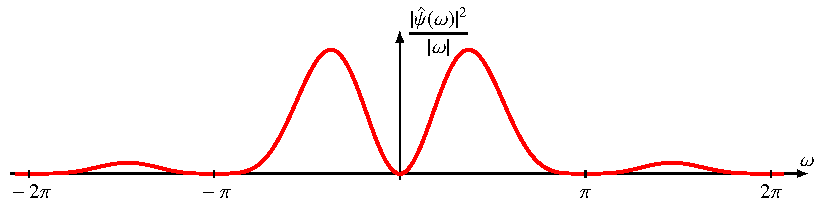
\includegraphics{chapters/4-cwt/images/hatpsi.pdf}
\caption{Nachweis der Zulässigkeitsbedingung für das Haar-Wavelet.
Die Funktion $|\hat{\psi}|^2/|\omega|$ ist besschränkt und fällt
für grosse $\omega$ wie $1/|\omega|^2$ ab, ihr Integral ist daher
beschränkt.
\label{cwt:figure:haarzulaessig}}
\end{figure}

Die Zulässigkeitsbedingung hat zur Folge, dass $\hat{\psi}(0)=0$ sein muss,
sofern dieser Funktionswert der Fouriertransformation überhaupt
definiert ist.
Das ist aber gleichbedeutend damit, dass 
\[
\int_{-\infty}^\infty \psi(t)\,dt = 0.
\]
Das Haar-Wavelet erfüllt diese letzte Eigenschaft.
Lässt sich daraus eventuell ein einfacher zu überprüfendes Kriterium
ableiten?
Tatsächlich gilt der folgende Satz

\begin{satz}
\label{satz:zulaessigkeit}
Ist $\psi \in L^2(\mathbb R)$ so, dass $t\psi\in L^1(\mathbb R)$, dann
ist die Zulässigkeitsbedingung gleichbedeutend mit
\[
\int_{-\infty}^\infty \psi(t)\,dt = 0
\qquad\text{oder gleichbedeutend}\qquad
\hat{\psi}(0)=0.
\]
\end{satz}

% XXX TODO: Beweis des Satzes siehe Blatter p. 54

Dieses Kriterium ist vor allem darum so nützlich, weil die Bedingung
$t\psi\in L^1(\mathbb R)$ für praktisch in Frage kommende Wavelets sehr
oft trivialerweise erfüllt ist.
Ein Wavelet mit kompaktem Träger verschwindet ausserhalb eines Intervalls
$[-M,M]$, daher wird 
\[
\int_{-\infty}^\infty |t|\,|\psi(t)|\,dt
\le 
M \int_{-M}^M |\psi(t)|\,dt < \infty.
\]
Darin haben wir die Aussagen von Satz~\ref{satz:l2inl1} verwendet,
dass $L^2$-Funktionen auf einem beschränkten Intervall integrierbar sind.
Ein weiterer interessanter Fall sind Wavelets, die für $t\to\infty$
sehr rasch abfallen, wie im folgenden Beispiel.

\begin{beispiel}
\begin{figure}
\centering
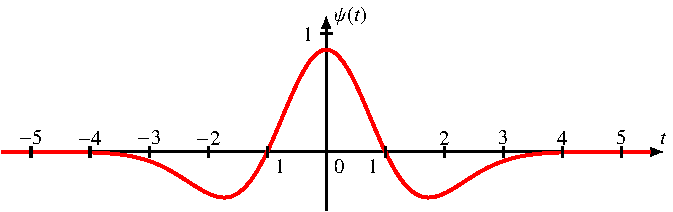
\includegraphics{chapters/4-cwt/images/mexican.pdf}
\caption{Mexikaner-Hut Wavelet gemäss
\eqref{wavelet:mexikanerhut}
\label{wavelet:mexikanerhut:graph}}
\end{figure}
Das Mexikanerhut-Wavelet ist definiert durch die Funktion
\begin{equation}
\psi_{\text{M}}(t) = \frac{2}{\pi^{\frac14}\sqrt{3}}(1-t^2) e^{-t^2/2}.
\label{wavelet:mexikanerhut}
\end{equation}
Der Faktor $e^{-t^2/2}$ fällt derart schnell ab, dass auch $|t|^k e^{-t^2/2}$
immer noch exponentiell schnell gegen Null abfällt.
Sein Graph ist dargestellt in Abbildung~\ref{wavelet:mexikanerhut:graph}.
Die Funktion $\psi_{\text{M}}$ ist zudem eine ungerade Funktion und %TODO: Mexikanerhut ist gerade.
erfüllt damit automatisch die Bedingung von Satz~\ref{satz:zulaessigkeit}.
\end{beispiel}

Das Kriterium von Satz~\ref{satz:zulaessigkeit} führt uns aber auch auf
das folgende Paradoxon. 
Da das Integral von $\psi$ verschwindet, dann auch von allen verschobenen
und skalierten Versionen von $\psi$, dann müsste doch auch die Grenzfunktion
diese Eigenschaft haben.
Wir werden später zeigen, dass die Approximationen der Ausgangsfunktion,
die mit der Wavelet-Transformation gewonnen wurden, zwar im Sinne von $L^2$
gegen die Ausgangsfunktion konvergieren, nicht aber im Sinne von $L^1$.



